% Packages %%%%%%%%%%%%%%%%%%%%%%%%%%%%%%%%%%%%%%%%%%%%%%%%%%%
\documentclass[conference]{IEEEtran}
\IEEEoverridecommandlockouts 
\usepackage{cite}
\usepackage[cmex10]{amsmath}
\usepackage{amssymb}
%\usepackage{algorithmic}
\usepackage{array}
\usepackage{mdwmath}
\usepackage{mdwtab}
\usepackage{eqparbox}
\usepackage{graphicx}
\usepackage[]{subfigure}
\usepackage{url}
\usepackage[algoruled,vlined,linesnumbered]{algorithm2e}
\usepackage{verbatim}
\usepackage{color}
\usepackage{hyperref}
\usepackage{mathtools}

\makeindex 
\makeatletter

%%%%%%%%%%%%%%%%%%%%%%%%%%%%%%%%%%%%%%%%%%%%%%%%%%%%%%%%%%%%%%%%
% Magic stuff to shrink stuff
\makeatletter
\renewcommand\section{\@startsection{section}{1}{\z@}
                                  {-3.0ex plus -1.5ex minus -0.5ex}
                                  {0.7ex plus 1ex minus 0ex}
                                  {\bfseries}}
\renewcommand\subsection{\@startsection{subsection}{1}{\z@}
                                  {-2.0ex plus -1.5ex minus -0.5ex}
                                  {0.7ex plus 1ex minus 0ex}
                                  {\itshape\bfseries}}
\makeatother


%\newcommand{\shrinka}{\def\baselinestretch{0.99}\large\normalsize}

\long\def\IGNORE#1{}

%%%%%%%%%%%%%%%%%%%%%%%%%%%%%%%%%%%%%%%%%%%%%%%%%%%%%%%%%%%%%%%%%%%
% New commands
\newcommand{\Disks}{\ensuremath{\mathcal{D}}}
\newcommand{\Container}{\ensuremath{\mathit{C}}}
\newcommand{\initMax}{r_{0}\_\text{\textit{Max}}}
\newcommand{\initMin}{r_{0}\_\text{\textit{Min}}}

%%%%%%%%%%%%%%%%%%%%%%%%%%%%%%%%%%%%%%%%%%%%%%%%%%%%%%%%%%%%
% Paper Info
\author{ Ana Huam\'{a}n Quispe% <-this % stops a space
  \thanks{The author is with the Georgia Institute of Technology, Atlanta, GA.{\tt\small ahuaman3@gatech.edu}}}
\title{ {ECE8843} {A}ssignment 3 : {R}obot {P}ath {P}lanning }  
%%%%%%%%%%%%%%%%%%%%%%%%%%%%%%%%%%%%%%%%%%%%%%%%%%%%%%%%%%%%
% Document
\begin{document}
\maketitle
%%%%%%%%%%%%%%%%%%%%%%%%%%%%%%%%%%%%%%%%%%%%%%%%%%%
%% Problem Statement
\section{Problem Statement}
\label{sec:ProbStatement}
Robbyna is a robot located in a known 2D environment. Having as
input data the start and goal location of the robot, as well as
its dimensions, find a path of waypoints $(x,y)$ to reach a 
given goal position.

The initial map is shown below:

%------------------------------------------------------------
% Image: World Map
\begin{figure}[h]
	\centering
	\fbox{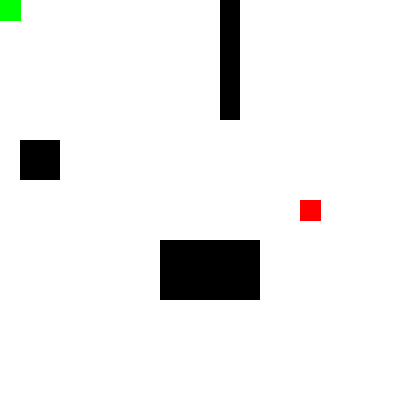
\includegraphics[width=0.9\columnwidth]{images/map_original.png}}	
	\caption{Original map}
	\label{fig:originalMap}
\end{figure} 

% ********************
\subsection{Initial Conditions}
\begin{itemize}
\item{ \textit{Start Location:} $(0,0)$ }
\item{ \textit{Goal Location:} $(15,10)$ }
\item{ \textit{Robot Dimensions:} $(1,1)$ }
\end{itemize}
 
and the obstacles are located as shown in Table \ref{tab:originalobstacles}

%--------------------------------------------
% Table: Original Obstacles
\begin{table}[h]
\centering
\caption{Original obstacles metrics}
\begin{tabular}{|c|c|c|}
\hline 
\textit{ \textbf{Obstacle}} & \textit{ \textbf{Original Location}} & \textit{ \textbf{Original Size}}\\
\hline 
0 & $(8, 12)$ & $(5, 3)$ \\
1 & $(1, 7)$ & $(2, 2)$ \\
2 & $(11, 0)$ & $(1, 6)$ \\ 
\hline
\end{tabular}
\label{tab:originalobstacles}
\end{table} 


% ********************
\subsection{Assumptions and definitions}
Since the problem statement does not pose any constraint on 
the robot's movement, I am assuming that the agent is capable
of omnidirectional movement.

We define each grid as having possibly one one out of 3 states:
\begin{itemize}
\item{ \textit{Free:} None of the area occupied by the grid is occupied 
by an obstacle}
\item{ \textit{Obstacle:} Some or all of the area occupied by the grid 
is part of an obstacle}
\item{ \textit{Inflated:} Space that cannot be reached by the robot and 
that is in the neighborhood of an obstacle}
\end{itemize}

%%%%%%%%%%%%%%%%%%%%%%%%%%%%%%%%%%%%%%%%%%%%%%%%%%%
%% Grown Map
\section{Obstacle Growing}
\label{sec:obstacleGrowing}
We implemented a simple function that grows the existing obstacles.
The function evaluates each grid on the 2D world. If the grid is
an \textit{obstacle}, then it will inflate the obstacle by setting 
the \textit{free} neighbors to an \textit{inflated} state.

The map with grown obstacles is shown in Fig.\ref{fig:grownObstaclesMap}.
The new dimensions of the obstacles are shown in Table \ref{tab:grownObstacles}.
In general the obstacles were inflated approx. 1 grid at each side (with the exception
of obstacles at the border of the map)

%--------------------------------------------
% Table: Grown Obstacles
\begin{table}[h]
\centering
\caption{Grown obstacles metrics}
\begin{tabular}{|c|c|c|}
\hline 
\textit{ \textbf{Obstacle}} & \textit{ \textbf{Location}} & \textit{ \textbf{Size}}\\
\hline 
0 & $(7, 11)$ & $(7, 5)$ \\
1 & $(0, 6)$ & $(4, 4)$ \\
2 & $(10, 0)$ & $(3, 7)$ \\ 
\hline
\end{tabular}
\label{tab:grownObstacles}
\end{table} 

%------------------------------------------------------------
% Image:Grown Obstacles
\begin{figure}[h]
	\centering
	\fbox{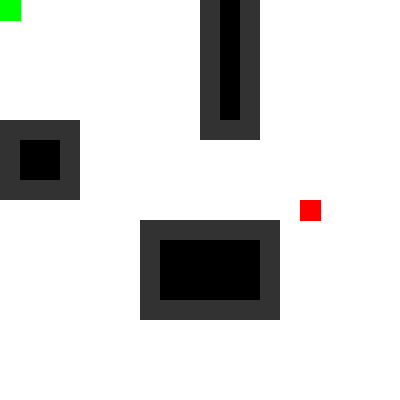
\includegraphics[width=0.9\columnwidth]{images/map_grownObstacles.png}}
	\caption{Map with grown obstacles}
	\label{fig:grownObstaclesMap}
\end{figure} 

%%%%%%%%%%%%%%%%%%%%%%%%%%%%%%%%%%%%%%%%%%%%%%%%%%%
%% Roadmap
\section{Probabilistic Random Map}
\label{sec:Roadmap}
After growing the obstacles we generated a roadmap to represent
our environment. Our method of choice was Probabilistic Roadmaps.
We generated a roadmap with $350$ random nodes, which produced a very dense map.
The edges in the map were generated by joining nodes with a distance
between them of less than $2.0$ grid units. We chose a small value 
to avoid having to test for collision along the edges.

The roadmap obtained can be seen in Fig.\ref{fig:roadmap}. Blue circles
represent the nodes and the magenta lines are the edges. The green
and red rectangles represent the start and goal location.

%------------------------------------------------------------
% Image:Roadmap
\begin{figure}[h]
	\centering
	\fbox{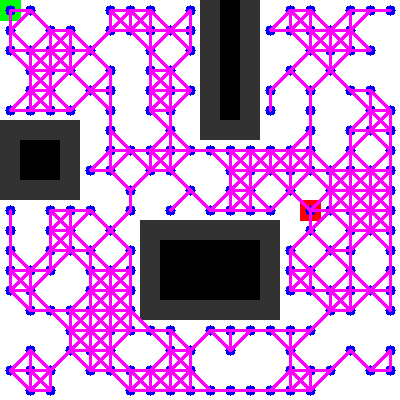
\includegraphics[width=0.9\columnwidth]{images/roadmap.png}}
	\caption{Roadmap with $350$ nodes}
	\label{fig:roadmap}
\end{figure} 

%%%%%%%%%%%%%%%%%%%%%%%%%%%%%%%%%%%%%%%%%%%%%%%%%%%
%% Path
\section{Path Search}
\label{sec:PathSearch}
The PRM generated in the previous section is nothing more than an
undirected graph composed of nodes and edges. To find the path between
the start and goal location, first we located the two nodes closest to 
the start and goal location and then performed a breadth-first search
between these nodes. Once found a path between these two, we just attached the original start
and end locations to the extremes of this path. Since our PRM is very dense,
the joining of these locations did not require collision checking.

Our breadth-first procedure assumed that all connected nodes had the same
distance with respect to their parent node. This is not exactly true, since
some children nodes where directly at the left, right, up or down directions 
of their parent, whereas other were at diagonal direction, hence their distances
were not the same. However, since these are small we decided not to assign them
different costs in order to preserve simplicity.

The path found is the green polyline depicted in Fig.\ref{fig:path}. The waypoints
that compound the path are shown in Table \ref{tab:waypoint}

%------------------------------------------------------------
% Image:Path Search
\begin{figure}[h]
	\centering
	\fbox{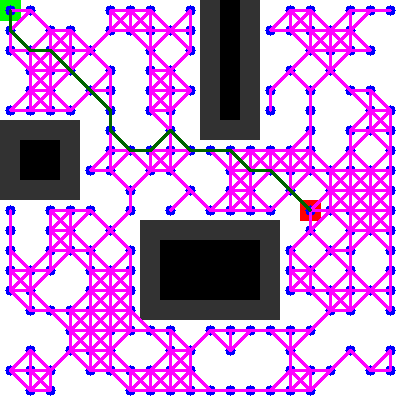
\includegraphics[width=0.9\columnwidth]{images/path.png}}
	\caption{Path found highlighted in green}
	\label{fig:path}
\end{figure} 

%--------------------------------------------
% Table: Waypoints
\begin{table}[h]
\centering
\caption{Waypoints}
\begin{tabular}{|c|c|}
\hline 
\textit{ \textbf{Waypoint}} & \textit{ \textbf{Location}} \\
\hline 
0 & $(0, 0)$ \\
1 & $(0, 1)$ \\
2 & $(1, 2)$ \\ 
3 & $(2, 2)$ \\ 
4 & $(3, 3)$ \\ 
5 & $(4, 4)$ \\ 
6 & $(5, 5)$ \\ 
7 & $(5, 6)$ \\
8 & $(6, 7)$ \\ 
9 & $(7, 7)$ \\ 
10 & $(8, 6)$ \\ 
11 & $(9, 7)$ \\ 
12 & $(10, 7)$ \\
13 & $(11, 7)$ \\
14 & $(12, 8)$ \\
15 & $(13, 8)$ \\
16 & $(14, 9)$ \\
17 & $(15, 10)$ \\
18 & $(15, 10)$ \\ 
\hline
\end{tabular}
\label{tab:waypoint}
\end{table} 

\end{document}